\documentclass[citecolor=blue,10pt]{beamer}
\usepackage{graphicx, color, booktabs}
\usepackage{ulem}
\usepackage{cancel}
\usepackage{lmodern}
\usepackage{natbib}
\usepackage{fancybox}
\usepackage{marvosym}
\usepackage{algorithm}
\usepackage{algorithmic}
%\usepackage{bbding}
%\usepackage[citecolor=blue]{hyperref}
\usepackage{textpos}
\hypersetup{
  colorlinks,
  citecolor=blue,
  linkcolor=black
}



%% maxwidth is the original width if it is less than linewidth
%% otherwise use linewidth (to make sure the graphics do not exceed the margin)

%\addtobeamertemplate{frametitle}{}{%
%\begin{textblock*}{200mm}(.8\textwidth,-0.5cm)
%\includegraphics[height=1cm,width=3cm]{ksu}
%\end{textblock*}}


\def\I{\mathbb{I}}

\def\bg{{\boldsymbol \gamma}}
\definecolor{fgcolor}{rgb}{0.2, 0.2, 0.2}
\def\R{\mathbb{R}}
\def\T{{ \mathrm{\scriptscriptstyle T} }}
\def\v{{\varepsilon}}
\def\uSigma{{\boldsymbol \Sigma}}
\newcommand{\uone} {\mbox{\boldmath$1$}}
\newcommand{\0} {\mbox{\boldmath$0$}}
\def\1{{\boldsymbol 1}}
\def\diag{{\rm diag}}
\newcommand{\uV} {{\boldsymbol V}}
\newcommand{\uv} {\mbox{\boldmath$v$}}
\newcommand{\uu} {\mbox{\boldmath$u$}}
\newcommand{\uH} {{\boldsymbol H}}
\newcommand{\uB} {{\boldsymbol B}}
\newcommand{\uD} {{\boldsymbol D}}
\newcommand{\uU} {{\boldsymbol U}}
\newcommand{\uC} {\mbox{\boldmath$C$}}
\newcommand{\uE} {\mbox{\boldmath$E$}}
\newcommand{\pkg}[1]{{\fontseries{b}\selectfont #1}} 
\newcommand{\uA}{{\boldsymbol A}}
\newcommand{\ua}{{\boldsymbol a}}
\newcommand{\uz}{{\boldsymbol z}}
\newcommand{\ub}{{\boldsymbol b}}
\newcommand{\uy}{{\boldsymbol y}}
\newcommand{\uo}{{\boldsymbol o}}
\newcommand{\uc}{{\boldsymbol c}}
\newcommand{\uY}{{\boldsymbol Y}}
\newcommand{\ux}{{\boldsymbol x}}
\newcommand{\uh}{{\boldsymbol h}}

\newcommand{\uX}{{\boldsymbol X}}
\newcommand{\uw} {\mbox{\boldmath$w$}}

\newcommand{\ug} {\mbox{\boldmath$g$}}
\newcommand{\uW} {\mbox{\boldmath$W$}}
\newcommand{\us} {\mbox{\boldmath$s$}}
\newcommand{\um} {\mbox{\boldmath$m$}}
\newcommand{\uF} {\mbox{\boldmath$F$}}
\newcommand{\uf} {\mbox{\boldmath$f$}}
\newcommand{\udelta} {\mbox{\boldmath$\delta$}}
\newcommand{\uDelta} {\mbox{\boldmath$\Delta$}}
\newcommand{\up} {{\boldsymbol p}}
\newcommand{\uP} {\mbox{\boldmath$P$}}
\newcommand{\uQ} {\mbox{\boldmath$Q$}}

\newcommand{\uK} {\mbox{\boldmath$K$}}
\newcommand{\uZ} {\mbox{\boldmath$Z$}}
\newcommand{\uI} {\mbox{\boldmath$I$}}
\newcommand{\utheta}{{\boldsymbol \theta}}

\newcommand{\uTheta} {\mbox{\boldmath $\Theta$}}
\newcommand{\umu} {{\boldsymbol \mu}}
\newcommand{\usig} {\mbox{\boldmath $\Sigma$}}
\newcommand{\ualpha} {\mbox{\boldmath $\alpha$}}
\newcommand{\ulambda}{{\boldsymbol \lambda}}
\newcommand{\ubeta}{{\boldsymbol \beta}}
\newcommand{\ueta} {\mbox{\boldmath $\eta$}}
\newcommand{\utau} {\mbox{\boldmath $\tau$}}
\newcommand{\ukappa} {\mbox{\boldmath $\kappa$}}
\newcommand{\uepsilon} {\mbox{\boldmath $\epsilon$}}
\newcommand{\uOmega} {\mbox{\boldmath $\Omega$}}
\renewcommand{\bibsection}{\vskip 5mm\centering{REFERENCES}}
\newcommand{\red}{\textcolor{red}}
\newcommand{\card}{{\rm card}}
\newcommand{\rank}{{\rm rank}}
\def\Sup{\operatornamewithlimits{sup\vphantom{p}}}
\def\mis{{\rm mis}}
\def\obs{{\rm obs}}
\def\full{{\rm full}}
\newcommand{\Nor}{\mathcal{N}}
\newcommand{\To}{\rightarrow}
\newcommand{\Car}{\mathds{1}}
\newcommand{\Inte}{\mathds{N}}
\newcommand{\LL}{\mathds{L}}
\newcommand{\Real}{\mathds{R}}
\newcommand{\Inter}{\mathds{Z}}
\newcommand{\Esp}{\mathds{E}}
\newcommand{\Var}{\mbox{Var}}
\newcommand{\Cov}{\mbox{Cov}}
\newcommand{\Probability}{\mathbb{P}}
\newcommand{\Loi}{\mathcal{L}}
\newcommand{\Dist}{\mathcal{D}}
%\newcommand{\bfS}{\mathbf{S}}
\newcommand{\bgamma}{\mbox{\boldmath $\gamma$}}
\newcommand{\bGamma}{\mbox{\boldmath $\Gamma$}}
\newcommand{\dint}{\displaystyle\int}
%\renewcommand{\thesection}{\arabic{section}}
%\renewcommand{\theequation}{\arabic{section}.\arabic{equation}}
%\renewcommand{\thetheorem}{\arabic{section}.\arabic{theorem}}
%\renewcommand{\theassumption}{\arabic{section}.\arabic{assumption}}
%\renewcommand{\theproposition}{\arabic{section}.\arabic{proposition}}
%\renewcommand{\thecorollary}{\arabic{section}.\arabic{corollary}}
%\renewcommand{\thelemma}{\arabic{section}.\arabic{lemma}}
%\renewcommand{\theexample}{\arabic{section}.\arabic{example}}
%\renewcommand{\theremark}{\arabic{section}.\arabic{remark}}
%\renewcommand{\thealgorithm}{\arabic{section}.\arabic{algorithm}}


\usepackage{framed}
\newtheorem{proposition}{Proposition}
\newtheorem{remark}{Remark}
\newtheorem{definition1}{What is BIG DATA?}
\newtheorem{remark1}{Big Data Challenge I}
\newtheorem{remark7}{Big Data Challenge II}
\newtheorem{remark2}{Bayesian perspective}
\newtheorem{remark3}{Data}
\newtheorem{remark4}{\textcolor{red}{Generalized} Bregman divergence clustering}
\newtheorem{remark5}{Bayesian clustering with high-dimensional covariates}
\newtheorem{remark6}{Bayesian functional clustering with high-dimensional covariates}
\definecolor{shadecolor}{rgb}{.97, .97, .97}
\definecolor{messagecolor}{rgb}{0, 0, 0}
\definecolor{warningcolor}{rgb}{1, 0, 1}
\definecolor{errorcolor}{rgb}{1, 0, 0}

\usepackage{alltt}
\mode<presentation>
\setbeamercovered{dynamic}
\usetheme{Boadilla}

\begin{document}

\title{Bayesian selection of best subsets in high-dimensional regression}
\author{\bf Shiqiang Jin}

\institute{Department of Statistics\\
Kansas State University, Manhattan, KS\\
\quad\\
\quad\\
{\color{blue} Joint work with} \\
\quad\\
{\bf Gyuhyeong Goh}\\ \quad\\ Kansas State University, Manhattan, KS
}

\date{July 31, 2019}

\begin{frame}
\titlepage
\end{frame}

%\begin{frame}<beamer>
%\frametitle{Outline}
%\tableofcontents
%\end{frame}

\section{Bayesian linear regression model in High-dimensional Data}
\begin{frame}{Bayesian linear regression model in High-dimensional Data}
\begin{itemize}\itemsep=5mm
\item Consider a linear regression model
\begin{eqnarray} \label{eq:1}
\uy=\uX\ubeta +\uepsilon,
\end{eqnarray}
where $\uy=(y_1,\ldots,y_n)^{\T}$ is a response vector, $\uX=(\ux_1,\ldots,\ux_p)\in\mathbb{R}^{n\times p}$ is a model matrix, $\ubeta=(\beta_1,\ldots, \beta_p)^\T$ is a coefficient vector and $\uepsilon \sim N(0,\sigma^2 I_n)$.
 \item We assume {\color{red}{$p>n$}}, i.e. High-dimensional data. 
 \item We assume only a few number of predictors are associated with the response, i.e. $\ubeta$ is {\color{red}{sparse}}.
 \end{itemize}
\end{frame}


 \begin{frame}{Bayesian linear regression model in High-dimensional Data}
\begin{itemize}\itemsep=5mm
\item To better explain the {\color{red}{sparsity}} of $\ubeta$, we introduce a latent index set $\bg \subset \{1,\ldots,p\}$ so that $\uX_{\bg}$ represents a sub-matrix of $\uX$ containing $\ux_j$, $j\in\bg$.
 \item e.g. $\bg=\{1,3,4\} \Rightarrow \uX_{\bg}=(\ux_1,\ux_3,\ux_4)$.
\item The full model in (\ref{eq:1}) can be reduced to
\begin{eqnarray}\label{eq:2}
\uy=\uX_{\bg}\ubeta_{\bg} +\uepsilon.
\end{eqnarray}
\end{itemize}
\end{frame}





\begin{frame}{Priors and marginal posterior distribution}


\begin{itemize}\itemsep=5mm
\item Our {\color{blue}{Research Goals}} are to obtain: 
\item [(i)] $k$ most important predictors out of $\binom{p}{k}$ candidate models; 
\item [(ii)] a single best model from among $2^p$ candidate models.
\pause
\item We consider 
\begin{eqnarray*}
 \ubeta_{\bg}|\sigma^2,\bg &\sim&\text{Normal}(0,\tau \sigma^2 \uI_{|\bg|} ),\\
 \sigma^2 &\sim& \text{Inverse-Gamma}(a_{\sigma}/2,b_{\sigma}/2),\\
 \pi(\bg) &\propto& \mathbb{I}(|\bg|=k),
\end{eqnarray*}
where $|\bg|$ is number of elements in $\bg$.
\end{itemize}
\end{frame}

\begin{frame}{Priors and marginal posterior distribution }
\begin{itemize}\itemsep=5mm

\item Given $k$, it can be shown that 
\begin{eqnarray*}
\pi(\bg|\uy)&\propto&  \frac{(\tau^{-1})^{\frac{|\bg|}{2}}}{|\uX_{\bg}^{\T}
 \uX_{\bg}+\tau^{-1}\uI_{|\bg|} |^{\frac{1}{2}}  \left(\uy^{\T}\uH_{\bg}
 \uy+b_{\sigma}\right)^{\frac{a_{\sigma}+n}{2}  } }\mathbb{I}(|\bg|=k)\\
 &\equiv& {\color{red}{g(\bg)}}\mathbb{I}(|\bg|=k),
 \end{eqnarray*}
  where $\uH_{\bg} = \uI_n-\uX_{\bg}(\uX_{\bg}^{\T}\uX_{\bg}+\tau^{-1}\uI_{|\bg|})^{-1}\uX_{\bg}^{\T}$.
\item Hence, ${\color{red}{\Large g(\bg)}}$ is our {\color{red}{model selection criterion}}. 

\end{itemize}
\end{frame}

\begin{frame}{Best subset selection Algorithm}
\begin{itemize}\itemsep=5mm
\item Note that our {\color{red}{goals}} are to obtain {\color{red}{(i)}} $k$ most important predictors out of $\binom{p}{k}$ models; {\color{red}{(ii)}} a single best model from among $2^p$ candidate models.

\item Hence, this can be fallen into the description of {\color{red}{best subset selection}} as follows:
\end{itemize}
\begin{itemize}\itemsep=5mm
\pause
\item[(i)] Fixed size: for $k = 1,2,\ldots,p$,  select the best subset model by
  $$\mathcal{M}_k = \arg_{\bg}\max_{|\bg|=k}g(\bg)$$
from $\binom{p}{k}$ candidate models.
\item [(ii)] Varying size: Pick the single best model from $\mathcal{M}_1,\ldots,\mathcal{M}_p$.
\pause \item Challenge of best subset selection:\\
e.g. (i) $p=1000,k=5$, {\color{red}{$\binom{1000}{5}\approx8\times 10^{12}$}}; (ii) $p=40$, {\color{red}{$2^{40}\approx 10^{12}$}}.
\end{itemize}
\end{frame}
\begin{frame}{Neighborhood Search}
\begin{itemize}
\item To avoid the exhaustive computation, we resort to the idea of {\color{red}{Neighborhood Search}} proposed by \citet{Madigan1995} and \citet{hans2007}.
\item Let $\bg^{(t)}$ be a current state of $\bg$, $|\bg^{(t)}|=k$ is model size.
\item {\color{red}{Addition}} neighbor: $\mathcal{N}_{{\color{red}{\boldsymbol{+}}}} (\bg^{(t)})=\{\bg^{(t)} \cup \{j\}: j\notin \bg^{(t)}\}$; {\color{red}{model size?}} \\ \vspace{3mm}
\item {\color{red}{Deletion}} neighbor: $\mathcal{N}_{{\color{red}{\boldsymbol{-}}}}(\bg^{(t)})=\{\bg^{(t)} \setminus \{j'\}: j'\in \bg^{(t)}\}$; {\color{red}{model size?}}\vspace{3mm}

\item e.g. Suppose $p=4,k=2$. Let $\bg^{(t)} =\{1,2\}$, then
\begin{eqnarray*}
\mathcal{N}_+(\bg^{(t)}) &=& \{\{1,2,3\},\{1,2,4\}\},\\
\mathcal{N}_-(\bg^{(t)})&=& \{\{1\},\{2\}\}.
\end{eqnarray*}
\end{itemize}
\end{frame}
\begin{frame}{Hybrid best subset search with a fixed $k$}

\begin{itemize}\itemsep=2mm
  \item  Note our {\color{red}{Goal (i)}} is to find  $\hat\bg = \arg_{\bg}\max_{|\hat\bg|=k}g(\bg)$. 
  \item[1.] Initialize $\hat{\bg}$ s.t. $|\hat{\bg}|=k$.
  \item[2.] \textbf{Repeat} \quad  \texttt{\textcolor{blue}{\#deterministic search:local optimum}}
        \begin{itemize}\itemsep=2mm
         \item[] Update $\tilde{\bg }\leftarrow \arg\max_{\bg  \in \mathcal{N}_+(\hat{\bg} ) } g(\bg)$ ;\quad  \texttt{\textcolor{blue}{\# $\mathcal{N}_+(\hat{\bg})=\{\hat{\bg} \cup \{j\}: j\notin \hat{\bg} \}$}}
         \item[] Update $\hat{\bg}\leftarrow  \arg\max_{\bg  \in \mathcal{N}_-(\tilde{\bg} ) } g(\bg);$ \quad \texttt{\textcolor{blue}{\# $\mathcal{N}_-(\tilde{\bg })= \{\tilde{\bg } \setminus \{j\}: j\in \tilde{\bg } \}$}}
        \end{itemize}
  \item[] \textbf{until} convergence.
  \pause
\item In Step 2, we have $p+1$ many candidate models in all $\bg \in \mathcal{N}_+(\hat{\bg})$ and all $\bg \in \mathcal{N}_-(\tilde{\bg}))$ in each iteration.
\item compute $g(\bg)$ $p+1$ times in each iteration. 
\end{itemize}
\end{frame}


\begin{frame}{1st Key features of proposed algorithm}
\begin{eqnarray*}
g(\bg)=\frac{(\tau^{-1})^{\frac{|\bg|}{2}}}{{\color{red}{|\uX_{\bg}^{\T}
 \uX_{\bg}+\tau^{-1}\uI_{|\bg|} |^{\frac{1}{2}}}}  \left(\uy^{\T}\uH_{\bg}
 \uy+b_{\sigma}\right)^{\frac{a_{\sigma}+n}{2}}},
\end{eqnarray*}
where $\uH_{\bg} = \uI_n-\uX_{\bg}{\color{red}{(\uX_{\bg}^{\T}\uX_{\bg}+\tau^{-1}\uI_{|\bg|})^{-1}}}\uX_{\bg}^{\T}$.
\begin{itemize}
\item compute inverse matrix and determinant $p+1$ times. 
\item We propose the following formula and we can show that evaluating all candidate models in addition neighbor can be done \textcolor{red}{simultaneously} in this single computation. 
\begin{eqnarray}
\nonumber \ug({\mathcal{N}_+({\hat\bg})})&=& \left\{(\uy^{\T}\uH_{\hat{\bg}}\uy+b_{\sigma}) \1_p-\frac{(\uX^{\T}\uH_{\hat{\bg}}\uy)^2}{\tau^{-1}\1_p+\diag(\uX^{\T}\uH_{\hat{\bg}}\uX) } \right\}^
 {-\frac{a_{\sigma}+n}{2}}\times\\
 &&\left\{\tau^{-1} \1_p  +\diag(\uX^{\T}\uH_{\hat{\bg}}\uX) \right\}^{-1/2},
 \end{eqnarray}
 \item Similarly for $\ug({\mathcal{N}_-({\hat\bg})})$.
\end{itemize}
\end{frame}
\begin{frame}{Hybrid best subset search with a fixed $k$}
\begin{itemize}
  \item  Note our {\color{red}{Goal (i)}} is to find  $\hat\bg = \arg_{\bg}\max_{|\hat\bg|=k}g(\bg)$. 
  \item[1.] Initialize $\hat{\bg}$ s.t. $|\hat{\bg}|=k$.
  \item[2.] \textbf{Repeat} \quad  \texttt{\textcolor{blue}{\#deterministic search:local optimum}}
        \begin{itemize}\itemsep=2mm
         \item[] Update $\tilde{\bg }\leftarrow \arg\max \ug(\mathcal{N}_+(\hat{\bg} ) )$ ;\quad  \texttt{\textcolor{blue}{\# $\mathcal{N}_+(\hat{\bg})=\{\hat{\bg} \cup \{j\}: j\notin \hat{\bg} \}$}}
         \item[] Update $\hat{\bg}\leftarrow  \arg\max \ug( \mathcal{N}_-(\tilde{\bg} ) );$ \quad \texttt{\textcolor{blue}{\# $\mathcal{N}_-(\tilde{\bg })= \{\tilde{\bg } \setminus \{j\}: j\in \tilde{\bg } \}$}}
        \end{itemize}
  \item[] \textbf{until} convergence.
 \pause \item[3.] Set $\bg^{(0)}=\hat{\bg}$.
  \item[4.] \textbf{Repeat} for $t=1,\ldots,T$:  \quad  \texttt{\textcolor{blue}{\#stochastic search:global optimum}}
        \begin{itemize}\itemsep=2mm
         \item[] Sample $\bg^{*} \sim\pi (\bg |\uy)=\frac{\{g(\bg)\}}{\sum_{\bg}\{g(\bg)\}}\mathbb{I}\{\bg\in \mathcal{N}_+({\bg^{(t-1)}} ) \}$; 
         \item[] Sample $\bg^{(t)}\sim \pi (\bg |\uy)=\frac{\{g(\bg)\}}{\sum_{\bg}\{g(\bg)\}} \mathbb{I}\{\bg\in \mathcal{N}_-({\bg^{*}} ) \}$;
         \item[] \textbf{If} $\pi(\hat{\bg} |\uy)<\pi({\bg}^{(t)} |\uy)$, \textbf{then} update $\hat{\bg}=\bg^{(t)}$, break the loop, and go to 2.
        \end{itemize}
  \item[5.] Return $\hat{\bg}$.
  \item Note that all $g(\bg)$ are computed simultaneously in their neighbor space. 
 \end{itemize}
\end{frame}


\begin{frame}{2nd Key features of proposed algorithm}
\begin{itemize}\itemsep=5mm
\item To avoid staying in the local optimum for a long time in step 4, we use the {\color{red}{escort distribution}}.
\item The idea of {\color{red}{escort distribution}} (used in statistical physics and thermodynamics) is introduced to stimulate the movement of Markov chain.
\item An escort distribution of $g(\bg)$ is given as 
$$  \frac{\{g(\bg)\}^\alpha}{\sum_{\bg}\{g(\bg)\}^\alpha}, \alpha\in[0,1]$$
\end{itemize}
\end{frame}
\begin{frame}{Escort distributions}
\begin{itemize}

\item e.g. Consider 3 candidate models with its probability: 
\item If $\alpha=1,$
\end{itemize}
$$\frac{\{g(\bg)\}^\alpha}{\sum_{\bg}\{g(\bg)\}^\alpha}=\begin{cases} 0.02\quad & \text{model 1} \\ 0.90~\quad &\text{model 2} \\0.08~\quad &\text{model 3} \end{cases}.$$
\begin{figure}
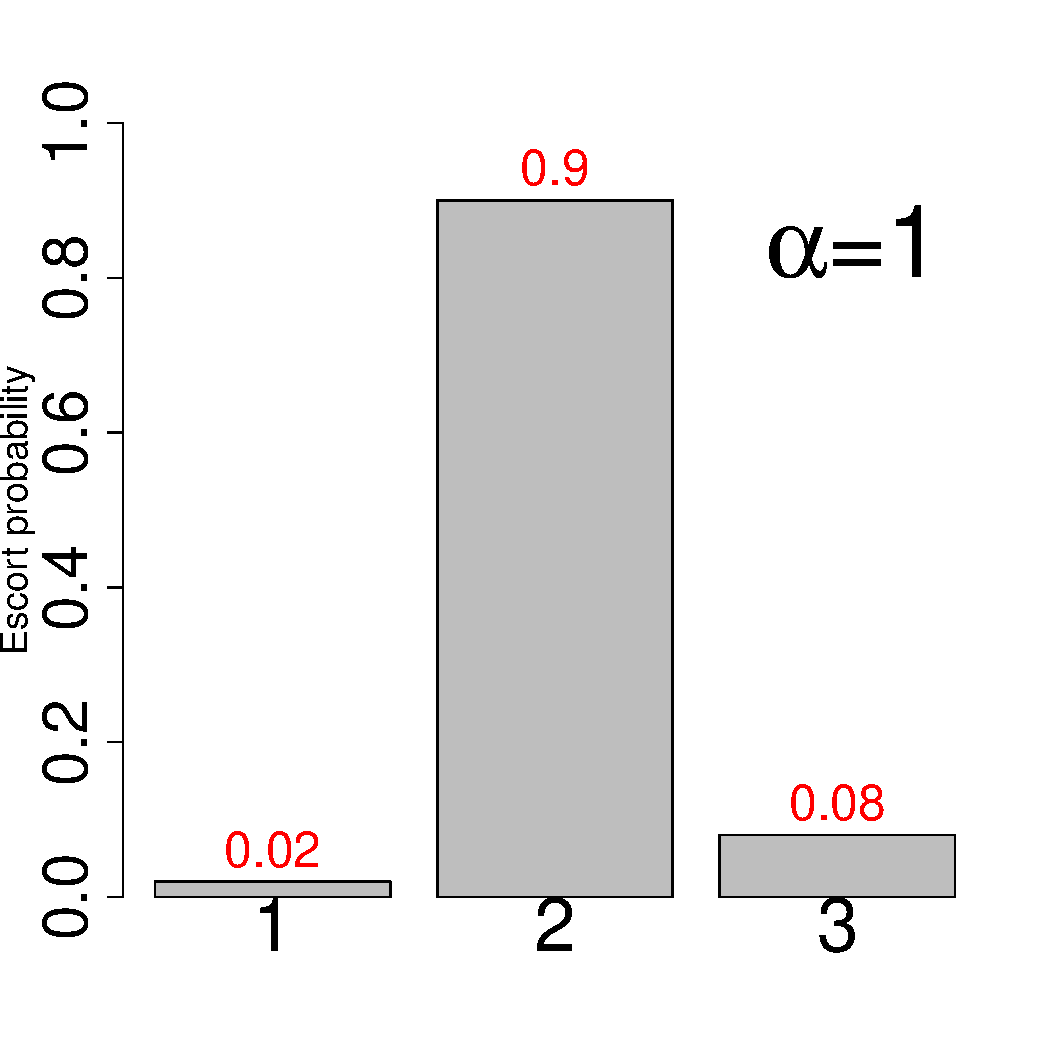
\includegraphics[trim=5mm 5mm 0 5mm,width=0.3\textwidth]{escort_fig1.pdf}
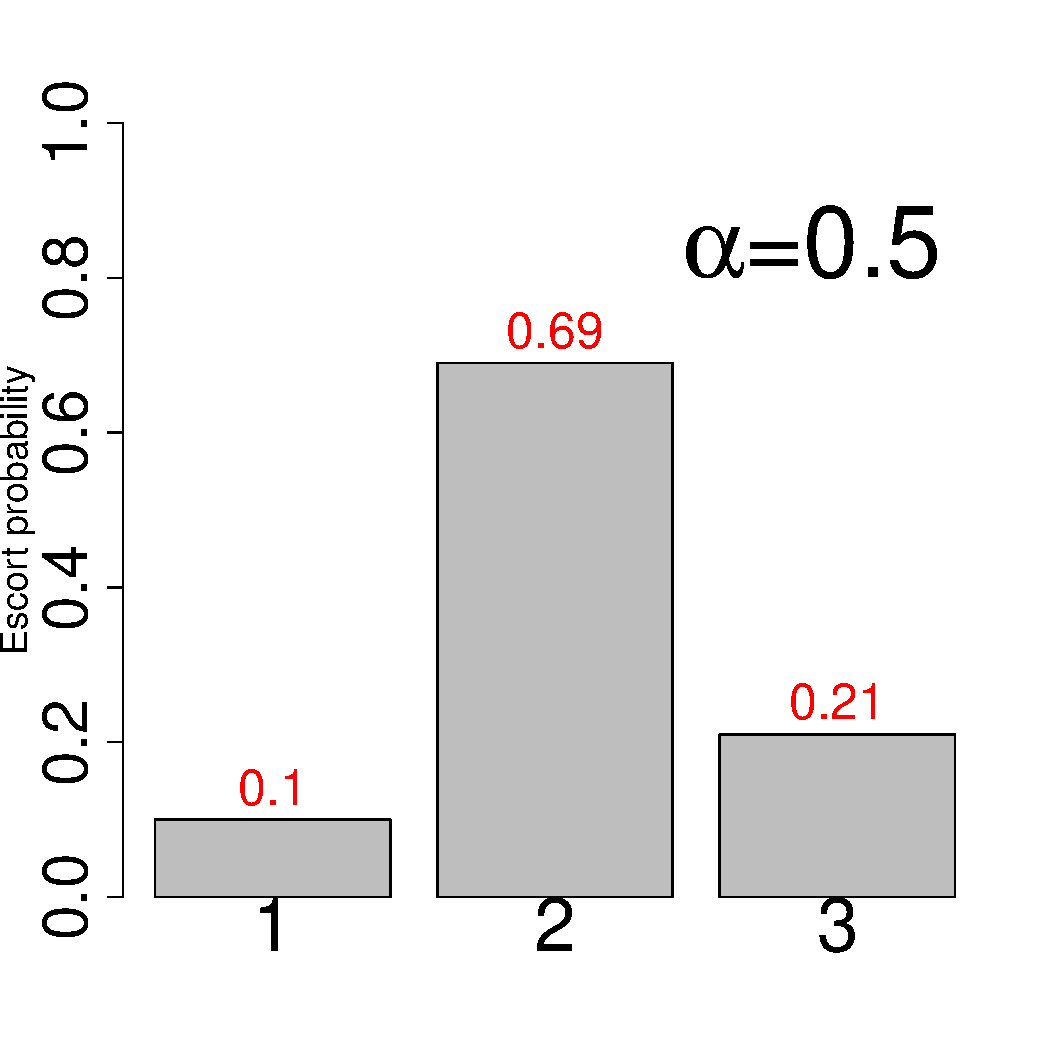
\includegraphics[trim=5mm 5mm 0 5mm,width=0.3\textwidth]{escort_fig2.pdf}
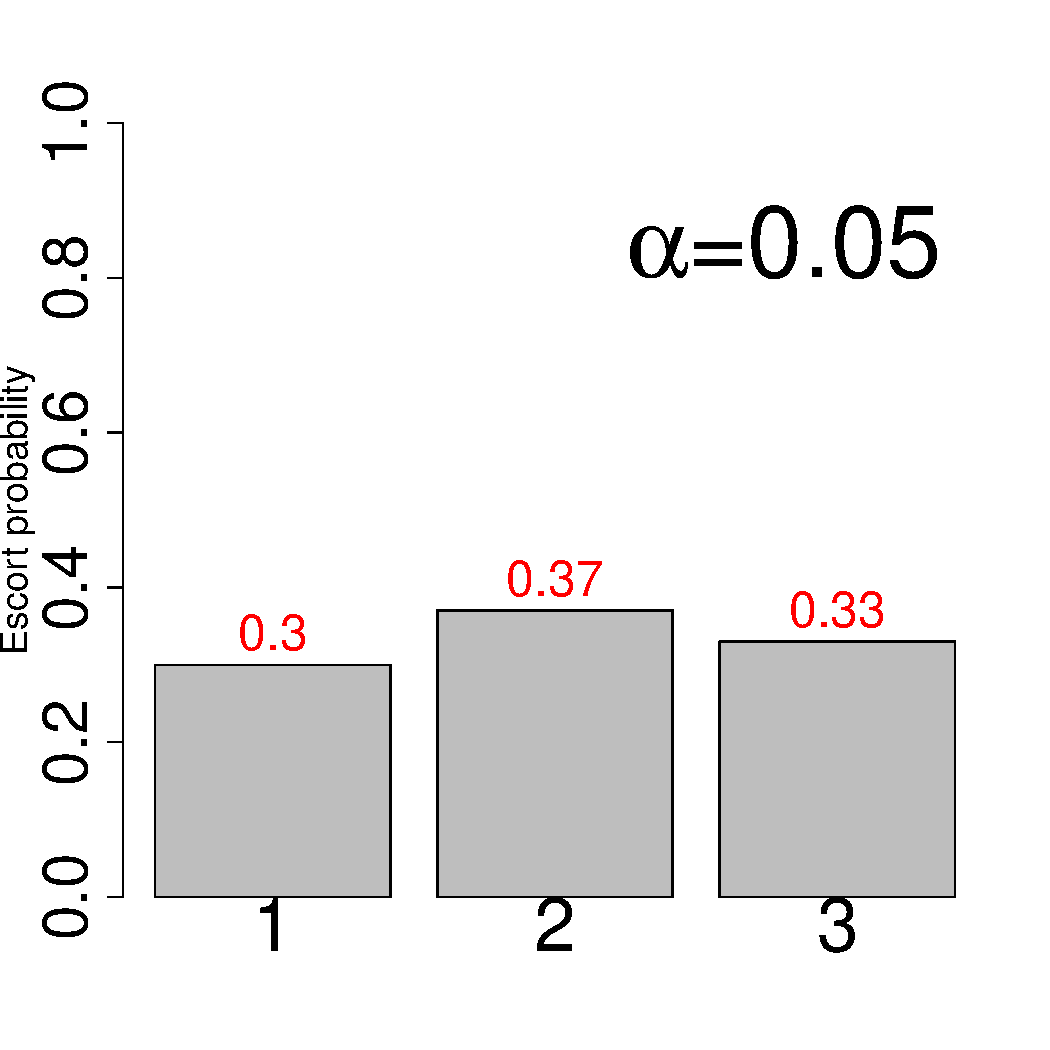
\includegraphics[trim=5mm 5mm 0 5mm,width=0.3\textwidth]{escort_fig3.pdf}
\caption{Escort distributions of $\pi_\alpha (\bg |\uy)$.}
\end{figure}
\end{frame}

\begin{frame}{Hybrid best subset search with a fixed $k$}
\begin{itemize}
  \item  Note our {\color{red}{Goal (i)}} is to find  $\hat\bg = \arg_{\bg}\max_{|\hat\bg|=k}g(\bg)$. 
  \item[1.] Initialize $\hat{\bg}$ s.t. $|\hat{\bg}|=k$.
  \item[2.] \textbf{Repeat} \quad  \texttt{\textcolor{blue}{\#deterministic search:local optimum}}
        \begin{itemize}\itemsep=2mm
         \item[] Update $\tilde{\bg }\leftarrow \arg\max \ug(\mathcal{N}_+(\hat{\bg} ) )$ ;\quad  \texttt{\textcolor{blue}{\# $\mathcal{N}_+(\hat{\bg})=\{\hat{\bg} \cup \{j\}: j\notin \hat{\bg} \}$}}
         \item[] Update $\hat{\bg}\leftarrow  \arg\max \ug( \mathcal{N}_-(\tilde{\bg} ) );$ \quad \texttt{\textcolor{blue}{\# $\mathcal{N}_-(\tilde{\bg })= \{\tilde{\bg } \setminus \{j\}: j\in \tilde{\bg } \}$}}
        \end{itemize}

  \item[] \textbf{until} convergence.
 \item[3.] Set $\bg^{(0)}=\hat{\bg}$.
  \item[4.] \textbf{Repeat} for $t=1,\ldots,T$:  \quad  \texttt{\textcolor{blue}{\#stochastic search:global optimum}}
        \begin{itemize}\itemsep=2mm
         \item[] Sample $\bg^{*} \sim\pi_\alpha (\bg |\uy)={\color{red}{\frac{\{g(\bg)\}^\alpha}{\sum_{\bg}\{g(\bg)\}^\alpha}}}\mathbb{I}\{\bg\in \mathcal{N}_+({\bg^{(t-1)}} ) \}$;  \quad  \texttt{\textcolor{blue}{\# $\alpha \in [0,1]$}}
         \item[] Sample $\bg^{(t)}\sim \pi_\alpha (\bg |\uy)={\color{red}{\frac{\{g(\bg)\}^\alpha}{\sum_{\bg}\{g(\bg)\}^\alpha}}} \mathbb{I}\{\bg\in \mathcal{N}_-({\bg^{*}} ) \}$;
         \item[] \textbf{If} $\pi(\hat{\bg} |\uy)<\pi({\bg}^{(t)} |\uy)$, \textbf{then} update $\hat{\bg}=\bg^{(t)}$, break the loop, and go to 2.
        \end{itemize}
  \item[5.] Return $\hat{\bg}$.
  \item Note that all $g(\bg)$ are computed simultaneously in their neighbor space. 
 \end{itemize}
\end{frame}
\begin{frame}{Best subset selection with varying $k$}
Note that {\color{red}{Goal (ii)}}: a single best model from among $2^p$ candidate models.
\begin{itemize}\itemsep=8mm
\item We extend "fixed" $k$ to varying $k$ by assigning a prior on $k$.
\item Note that the uniform prior, $k \sim \text{Uniform}\{1,\ldots,K\}$, tends to assign larger probability to a larger subset (see \citet{chen2008extended}). 
\item We define
$$\pi(k)\propto 1/\binom{p}{k} \mathbb{I}(k\leq K).$$
\end{itemize}
\end{frame}


\begin{frame}{Hybrid best subset search with varying $k$}
\begin{itemize}\itemsep=3mm
\item Bayesian best subset selection can be done by maximizing
\begin{eqnarray} 
\pi(\bg,k|\uy) \propto {\color{red}{g(\bg)/\binom{p}{k}}}
\end{eqnarray}
over $(\bg,k)$.
\item Our algorithm proceeds as follows:\\

 \begin{itemize}\itemsep=3mm
  \item[1.] \textbf{Repeat} for $k=1,\ldots,K$:
        
 Given $k$, implement the hybrid search algorithm to obtain best subset model $\hat\bg_k$.
        
  \item[2.] Find the best model $\hat\bg^*$ obtained by 
\begin{eqnarray} 
\hat\bg^*=\arg\max_{k\in\{1,\ldots,K \}}\left({\color{red}{g(\hat\bg_k)/\binom{p}{k}}}\right).
\end{eqnarray}
\end{itemize}

\end{itemize}
\end{frame}

\begin{frame}{Consistency of model selection criterion}
\begin{theorem}\label{thm:2} Let $\bg_*$ indicate the true model. Define $\Gamma=\{\bg:|\bg|\leq K,\bg\neq \bg_*\}$. Assume that $p=O(n^\xi)$ for $\xi\geq 1$. Under the asymptotic identifiability condition of \citet{chen2008extended}, if $\tau\to \infty$ as $n\to \infty$ but $\tau=o(n)$, then the proposed Bayesian subset selection possesses the Bayesian model selection consistency, that is,
\begin{eqnarray}\label{thm:2:eq}
\pi(\bg_*|\uy) > \max_{ \bg \in \Gamma }\pi(\bg|\uy)
\end{eqnarray}
in probability as $n\to \infty$.
\end{theorem}
\begin{itemize}
  \item As $n\to \infty$, the maximizer of $\pi(\bg|\uy)$ is the true model based on our model selection criterion.
\end{itemize}
\end{frame}
\begin{frame}{Simulation study}{Setup}
\begin{itemize}\itemsep=3mm
\item For given $n=100$, we generate the data from 
$$y_i\overset{ind}{\sim}\text{Normal}\left(\sum_{j=1}^p \beta_j x_{ij},1\right),$$
where 
\begin{itemize}\itemsep=3mm
\item $(x_{i1},\ldots,x_{ip})^\T \overset{iid}{\sim}\text{Normal}(\0_p,\uSigma)$ with $\uSigma=(\Sigma_{ij})_{p\times p}$ and $\Sigma_{ij}=\rho^{|i-j|}$,
\item $\beta_j \overset{iid}{\sim} \text{Uniform}\{-1,-2,1,2\}$ if $j\in \bg$ and $\beta_j=0$ if $j\notin \bg$. 
\item $\bg$ is an index set of size $4$ randomly selected from $\{1,2,\ldots,p\}$.
\item We consider four scenarios for $p$ and $\rho$: \\
(i) $p=200$, $\rho=0.1$, (ii) $p=200$, $\rho=0.9$,\\
 (iii) $p=1000$, $\rho=0.1$, (iv) $p=1000$, $\rho=0.9$. 
\end{itemize}
\end{itemize}
\end{frame}


\begin{frame}{Simulation study}{Results (high-dimensional scenarios)}
{\footnotesize
\begin{table}[H]
 \centering 
 \caption{$2,000$ replications; FDR (false discovery rate), TRUE\% (percentage of the true model detected), SIZE (selected model size), HAM (Hamming distance).}\label{T:sim1}
 \begin{tabular}{cc|c|c|c|c}
  \hline
  Scenario & Method                         & FDR  (s.e.)    & TRUE\% (s.e.)   & SIZE (s.e.)     & HAM (s.e.)    \\
  \hline
$p=200$ & {\color{red}{Proposed}} & 0.006 (0.001)  & 96.900 (0.388)  & 4.032 (0.004)    & 0.032 (0.004) \\
$\&\rho=0.1$& SCAD                           & 0.034 (0.002)  & 85.200 (0.794)  & 4.188 (0.011)   & 0.188 (0.011) \\
           & MCP                            & 0.035 (0.002)  & 84.750 (0.804)  & 4.191 (0.011)   & 0.191 (0.011) \\
           & ENET                           & 0.016 (0.001)  & 92.700 (0.582)  & 4.087 (0.007)   & 0.087 (0.007) \\
           & LASSO                          & 0.020 (0.002)  & 91.350 (0.629)  & 4.109 (0.009)   & 0.109 (0.009) \\
  \hline
$p=200$           & {\color{red}{Proposed}} & 0.023  (0.002) & 88.750  (0.707) & 3.985 (0.006)  & 0.203 (0.014) \\
$\&\rho=0.9$ & SCAD                           & 0.059 (0.003)  & 74.150 (0.979)  & 4.107 (0.015)   & 0.480 (0.022) \\
           & MCP                            & 0.137 (0.004)  & 55.400 (1.112)  & 4.264 (0.020)   & 1.098 (0.034) \\
           & ENET                           & 0.501 (0.004)  & 0.300 (0.122)   & 7.716 (0.072)   & 5.018 (0.052) \\
           & LASSO                          & 0.276 (0.004)  & 15.550 (0.811)  & 5.308 (0.033)   & 2.038 (0.034) \\
  \hline
 \end{tabular}
\end{table}}
\end{frame}



\begin{frame}{Simulation study}{Results (ultra high-dimensional scenarios)}
{\footnotesize
\begin{table}[H]
 \centering 
 \caption{$2,000$ replications; FDR (false discovery rate), TRUE\% (percentage of the true model detected), SIZE (selected model size), HAM (Hamming distance).}\label{T:sim2}
 \begin{tabular}{cc|c|c|c|c}
  \hline
  Scenario & Method                         & FDR  (s.e.)    & TRUE\% (s.e.)   & SIZE (s.e.)     & HAM (s.e.)    \\
  \hline
   $p=1000$        & {\color{red}{Proposed}} & 0.004 (0.001)   & 98.100 (0.305)  & 4.020 (0.003)    & 0.020 (0.003) \\
   $\&\rho=0.1$& SCAD                           & 0.027 (0.002)  & 87.900 (0.729)  & 4.145 (0.010)   & 0.145 (0.010) \\
           & MCP                            & 0.031 (0.002)  & 86.550 (0.763)  & 4.172 (0.013)   & 0.172 (0.013) \\
           & ENET                           & 0.035 (0.002)  & 84.850 (0.802)  & 4.181 (0.013)   & 0.206 (0.012) \\
           & LASSO                          & 0.014 (0.001)  & 93.850 (0.537)  & 4.073 (0.007)   & 0.073 (0.007) \\
  \hline
    $p=1000$       & {\color{red}{Proposed}} & 0.023(0.002)   & 89.850 (0.675)  & 4.005 (0.005) & 0.190 (0.013) \\
    $\&\rho=0.9$& SCAD                           & 0.068 (0.003)  & 74.250 (0.978)  & 4.196 (0.014)   & 0.493 (0.023) \\
           & MCP                            & 0.152 (0.004)  & 53.750 (1.115)  & 4.226 (0.017)   & 1.202 (0.035) \\
           & ENET                           & 0.417 (0.005)  & 0.150 (0.087)   & 6.228 (0.068)   & 4.089 (0.043) \\
           & LASSO                          & 0.265 (0.004)  & 19.500 (0.886)  & 5.139 (0.029)   & 1.909 (0.035) \\
  \hline
 \end{tabular}
\end{table}}
\end{frame}


\begin{frame}{Real data application}{Data description}
\begin{itemize}\itemsep=4mm
\item We apply the proposed method to Breast Invasive Carcinoma (BRCA) data generated by The Cancer Genome Atlas (TCGA) Research Network \url{http://cancergenome.nih.gov}. 
\item The data set contains $17,814$ gene expression measurements (recorded on the log scale) of $526$ patients with primary solid tumor. 
\item {\color{red}{BRCA1}} is a tumor suppressor gene and its mutations predispose women to breast cancer \citep{findlay2018accurate}. 

\end{itemize}
\end{frame}


\begin{frame}{Real data application}{Results (based on $4,000$ genes)}
\begin{itemize}
\item Our {\color{red}{goal}} here is to identify the best fitting model for estimating an association between BRCA1 (response variable) and the other genes (independent variables). 

$$\text{BRCA1} = \beta_1*\text{NBR2} + \beta_2*\text{DTL} + \ldots + \beta_p*\text{VPS25}+\uepsilon.$$
\item Results: 
\end{itemize}
\begin{table}[ht]
 \centering
 \caption{Model comparison}\label{T:realdata}
 \begin{tabular}{rrrrr}
  \hline
           & \# of selected  & PMSE & BIC     & EBIC    \\
  \hline
  {\color{red}{Proposed}} & 8 & 0.60      & 984.45  & 1099.50 \\
  SCAD     & 4 & 0.68      & 1104.69 & 1166.47 \\
  MCP      & 4 & 0.68      & 1104.69 & 1166.47 \\
  ENET     & 5 & 0.68      & 1110.65 & 1186.25 \\
  LASSO    & 4 & 0.68      & 1104.69 & 1166.47 \\
  \hline
 \end{tabular}
\end{table}
\end{frame}
\begin{frame}{Real data application}{Results (cont.)}
\begin{figure}
 \centering
 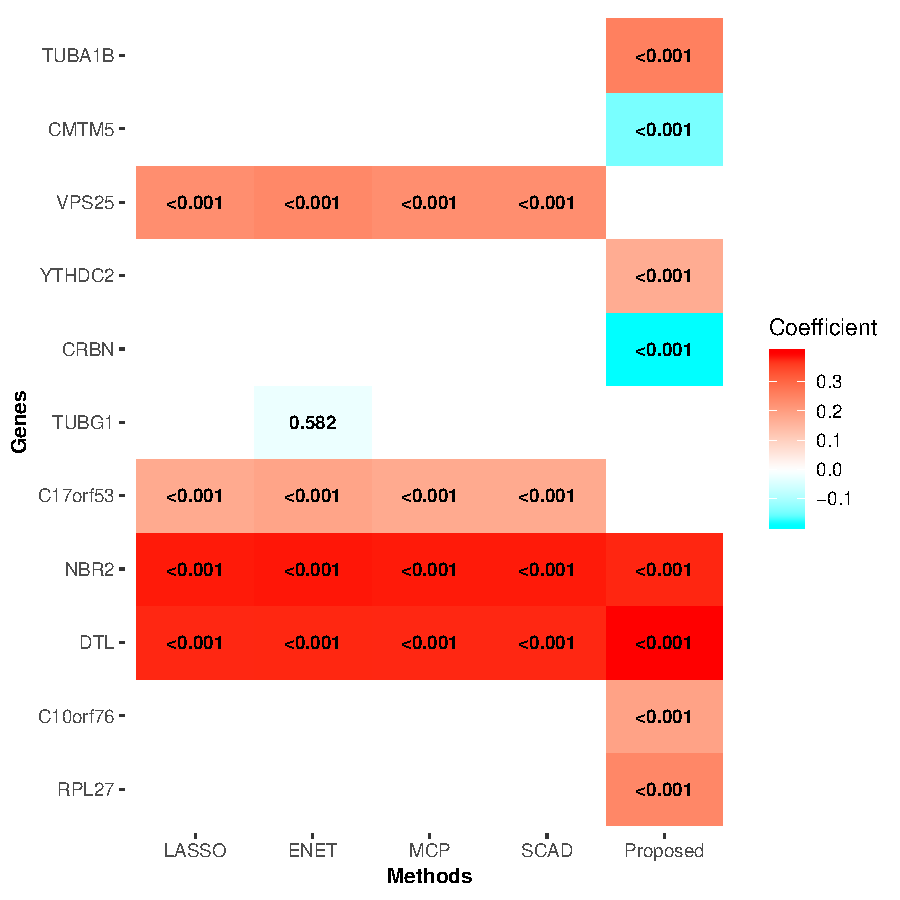
\includegraphics[width=0.6\textwidth,height=0.55\textwidth]{Heatmap.pdf}
 \caption{Except C10orf76, {\color{red}{7 genes}} are documented as {\color{red}{diseases-related genes}}}
\end{figure}

\end{frame}

\begin{frame}{Concluding remarks}
\begin{itemize}\itemsep=4mm
\item Parallel computing is applicable to our algorithm with varying $k$. 
\item The proposed method can be extended to multivariate linear regression models, binary regression models, and multivariate mixed responses models (in progress).
\end{itemize}

\end{frame}

\begin{frame}\footnotesize
%\bibliographystyle{biom}
%\bibliography{thesis_Goh}
\begin{thebibliography}{}
%\bibitem[\protect\citeauthoryear{Berg et al.}{Berg et al.}{2016}]{Berg:2016}
%Berg, E., Kim, J. K. and Skinner, C. (2016).
%\newblock Imputation under informative sampling
%\newblock {\em Journal of Survey Statistics and Methodology} {\bf }
%(In Press).

%\bibitem[\protect\citeauthoryear{Yin}{Yin}{2009}]{Yin:2009}
%Yin, G. (2009).
%\newblock Bayesian Generalized Method of Moments
%\newblock {\em Bayesian Analysis} {\bf 4,}
% 191--208.


%\bibitem[\protect\citeauthoryear{Xu, Chen and Mantel}{Xu, Chen and Mantel}{2013}]{Xu:2013}
%Xu, C., Chen, J., and Mantel, H. (2013).
%\newblock Pseudo-likelihood-based Bayesian information criterion for variable selection in survey data
%\newblock {\em Survey Methodology} {\bf 39,}
% 303--321.


%\bibitem[\protect\citeauthoryear{Li and Jiang}{Li and Jiang}{2014}]{Lin-Jiang:2014}
%Li, C. and Jiang, W. (2014).
%\newblock Model Selection for Likelihood-free Bayesian Methods Based on Moment Conditions: Theory and Numerical Examples
%\newblock {\em arXiv e-prints}.

%\bibitem[\protect\citeauthoryear{Schwarz}{Schwarz}{1978}]{Schwarz:1978}
%Schwarz, G. (1978).
%\newblock Estimating the dimension of a model.
%\newblock {\em The Annals of Statistics} {\bf 6,} 461--464.



%\bibitem[\protect\citeauthoryear{Tibshirani}{Tibshirani}{1996}]{tibshirani1996regression}
%Tibshirani, R. (1996).
%\newblock Regression shrinkage and selection via the lasso.
%\newblock {\em Journal of the Royal Statistical Society. Series B
%  (Methodological)\/}, 267--288.


\bibitem[\protect\citeauthoryear{Hans, Dobra, and West}{Hans et~al.}{2007}]{hans2007}
Hans, C., A.~Dobra, and M.~West (2007).
\newblock Shotgun stochastic search for ``large p'' regression.
\newblock {\em Journal of the American Statistical Association\/}~{\em
  102\/}(478), 507--516.


\bibitem[\protect\citeauthoryear{Chen and Chen}{Chen and
  Chen}{2008}]{chen2008extended}
Chen, J. and Z.~Chen (2008).
\newblock Extended bayesian information criteria for model selection with large
  model spaces.
\newblock {\em Biometrika\/}~{\em 95\/}(3), 759--771.


\bibitem[\protect\citeauthoryear{Findlay, Daza, Martin, Zhang, Leith,
  Gasperini, Janizek, Huang, Starita, and Shendure}{Findlay
  et~al.}{2018}]{findlay2018accurate}
Findlay, G.~M., R.~M. Daza, B.~Martin, M.~D. Zhang, A.~P. Leith, M.~Gasperini,
  J.~D. Janizek, X.~Huang, L.~M. Starita, and J.~Shendure (2018).
\newblock Accurate classification of brca1 variants with saturation genome
  editing.
\newblock {\em Nature\/}~{\em 562\/}(7726), 217.

\bibitem[\protect\citeauthoryear{Madigan, David, Jeremy York, and Denis Allard}{Madigan et~al.}{1995}]{Madigan1995}
Madigan, David, Jeremy York, and Denis Allard (1995).
\newblock Bayesian Graphical Models for Discrete Data.
\newblock {\em  International Statistical Review / Revue Internationale De Statistique\/}~{\em 63\/}(2), 215-232.



\end{thebibliography}
\end{frame}
%\bibliography{thesis_Goh}

\begin{frame}{Contact: \url{jinsq@ksu.edu}}
\vspace{2mm}
\centering \huge THANK YOU
\end{frame}

\end{document}